\section{Modules Explanation}

\subsection{\texttt{Control} Module}

\texttt{Control} module reads the $0..6$-th bits of the instruction as input, and outputs \texttt{ALUOp}, \texttt{ALUSrc}, \texttt{RegWrite}. The value of \texttt{RegWrite} is always $1$ (as every instruction in this homework needs to write register); the value of \texttt{ALUSrc} is $1$ for \texttt{addi}, \texttt{srai}, and $0$ otherwise, which is calculated by looking at the $5$-th bit of the instruction; the value of \texttt{ALUOp} is the $4, 5$-th bits of the instruction.

\subsection{\texttt{ALU\_Control} Module}

\texttt{ALU\_Control} module reads the $12..14, 25..31$-th bits of the instruction, \texttt{ALUOp} as input, and outputs \texttt{ALUOp3}, which will be used by \texttt{ALU} later. The module uses \texttt{ALUOp} to determine if the instruction is addi or srai, and then uses those $10$ bits of the instruction to determine what kind of instruction it is. The value of \texttt{ALUOp3} is as follow:\\
\texttt{0:and 1:xor 2:sll 3:add 4:sub 5:mul 6:srai}.

\subsection{\texttt{Sign\_Extend} Module}

\texttt{Sign\_Extend} module reads the $20..31$-th bits of the instruction, and outputs \texttt{res} (which is named \texttt{ext} in \texttt{CPU} module). The module sees those $12$ bits of the instruction as a sign integer (where the most significant bit is the sign bit), and extends this integer to $32$ bits by filling the $12..31$-th bits of \texttt{res} with the sign bit.

\subsection{\texttt{ALU} Module}

\texttt{ALU} module reads \texttt{a}, \texttt{b}, \texttt{op} (which is named \texttt{rs1}, \texttt{rs3}, \texttt{ALUOp3} in \texttt{CPU} module) as input, and outputs \texttt{c} (which is named \texttt{ALUres} in \texttt{CPU} module), \texttt{Zero}. The module uses \texttt{ALUOp3} to determine which operation should be done to \texttt{a}, \texttt{b}, and then calculates the result as \texttt{c}. The value of \texttt{Zero} is always $0$ (as the modules in this homework don't need the value of \texttt{Zero}).

\subsection{\texttt{Adder} Module}

\texttt{Adder} module reads \texttt{a}, \texttt{b} as input, and outputs \texttt{a}+\texttt{b} as \texttt{c}.

\subsection{\texttt{MUX32} Module}

\texttt{MUX32} module reads \texttt{a}, \texttt{b}, \texttt{sel} as input, and outputs \texttt{c}. The value of \texttt{c} is \texttt{a} if \texttt{sel} is $0$, and is \texttt{b} otherwise.

\subsection{\texttt{CPU} Module}

\texttt{CPU} module reads \texttt{clk\_i}, \texttt{rst\_i} as input, and does not output anything. The following are the things that is does:
\begin{enumerate}
\item It inputs \texttt{clk\_i}, \texttt{rst\_i}, \texttt{pc\_i} to \texttt{PC} module, and gets the output as \texttt{pc\_o}.
\item It inputs \texttt{pc\_o} to \texttt{Adder} module, and gets the output as \texttt{pc\_i}.
\item It inputs \texttt{pc\_o} to \texttt{Intruction\_Memory} module, and gets the output as \texttt{inst}.
\item It inputs \texttt{inst}[6:0] to \texttt{Control} module, and gets the output as \texttt{ALUOp}, \texttt{ALUSrc}, \texttt{RegWrite}.
\item It inputs \texttt{rst\_i}, \texttt{clk\_i}, \texttt{inst}[19:15], \texttt{inst}[24:20], \texttt{inst}[11:7], \texttt{ALUres}, \texttt{RegWrite} to \texttt{Registers} module, and gets the output as \texttt{rs1}, \texttt{rs2}.
\item It merges \texttt{inst}[31:25], \texttt{inst}[14:12] as \texttt{ALUinst}, inputs \texttt{ALUinst}, \texttt{ALUOp} to \texttt{ALU\_Control} module, and gets the output as \texttt{ALUOp3}.
\item It inputs \texttt{inst}[31:20] to \texttt{Sign\_Extend} module, and gets the output as \texttt{ext}.
\item It inputs \texttt{rs2}, \texttt{ext} to \texttt{MUX32} module, and gets the output as \texttt{rs3}.
\item It inputs \texttt{rs1}, \texttt{rs3}, \texttt{ALUOp3} to \texttt{ALU}, and gets the output as \texttt{ALUres}, \texttt{Zero}.
\end{enumerate}

The above things can be illustrated as follow:\\
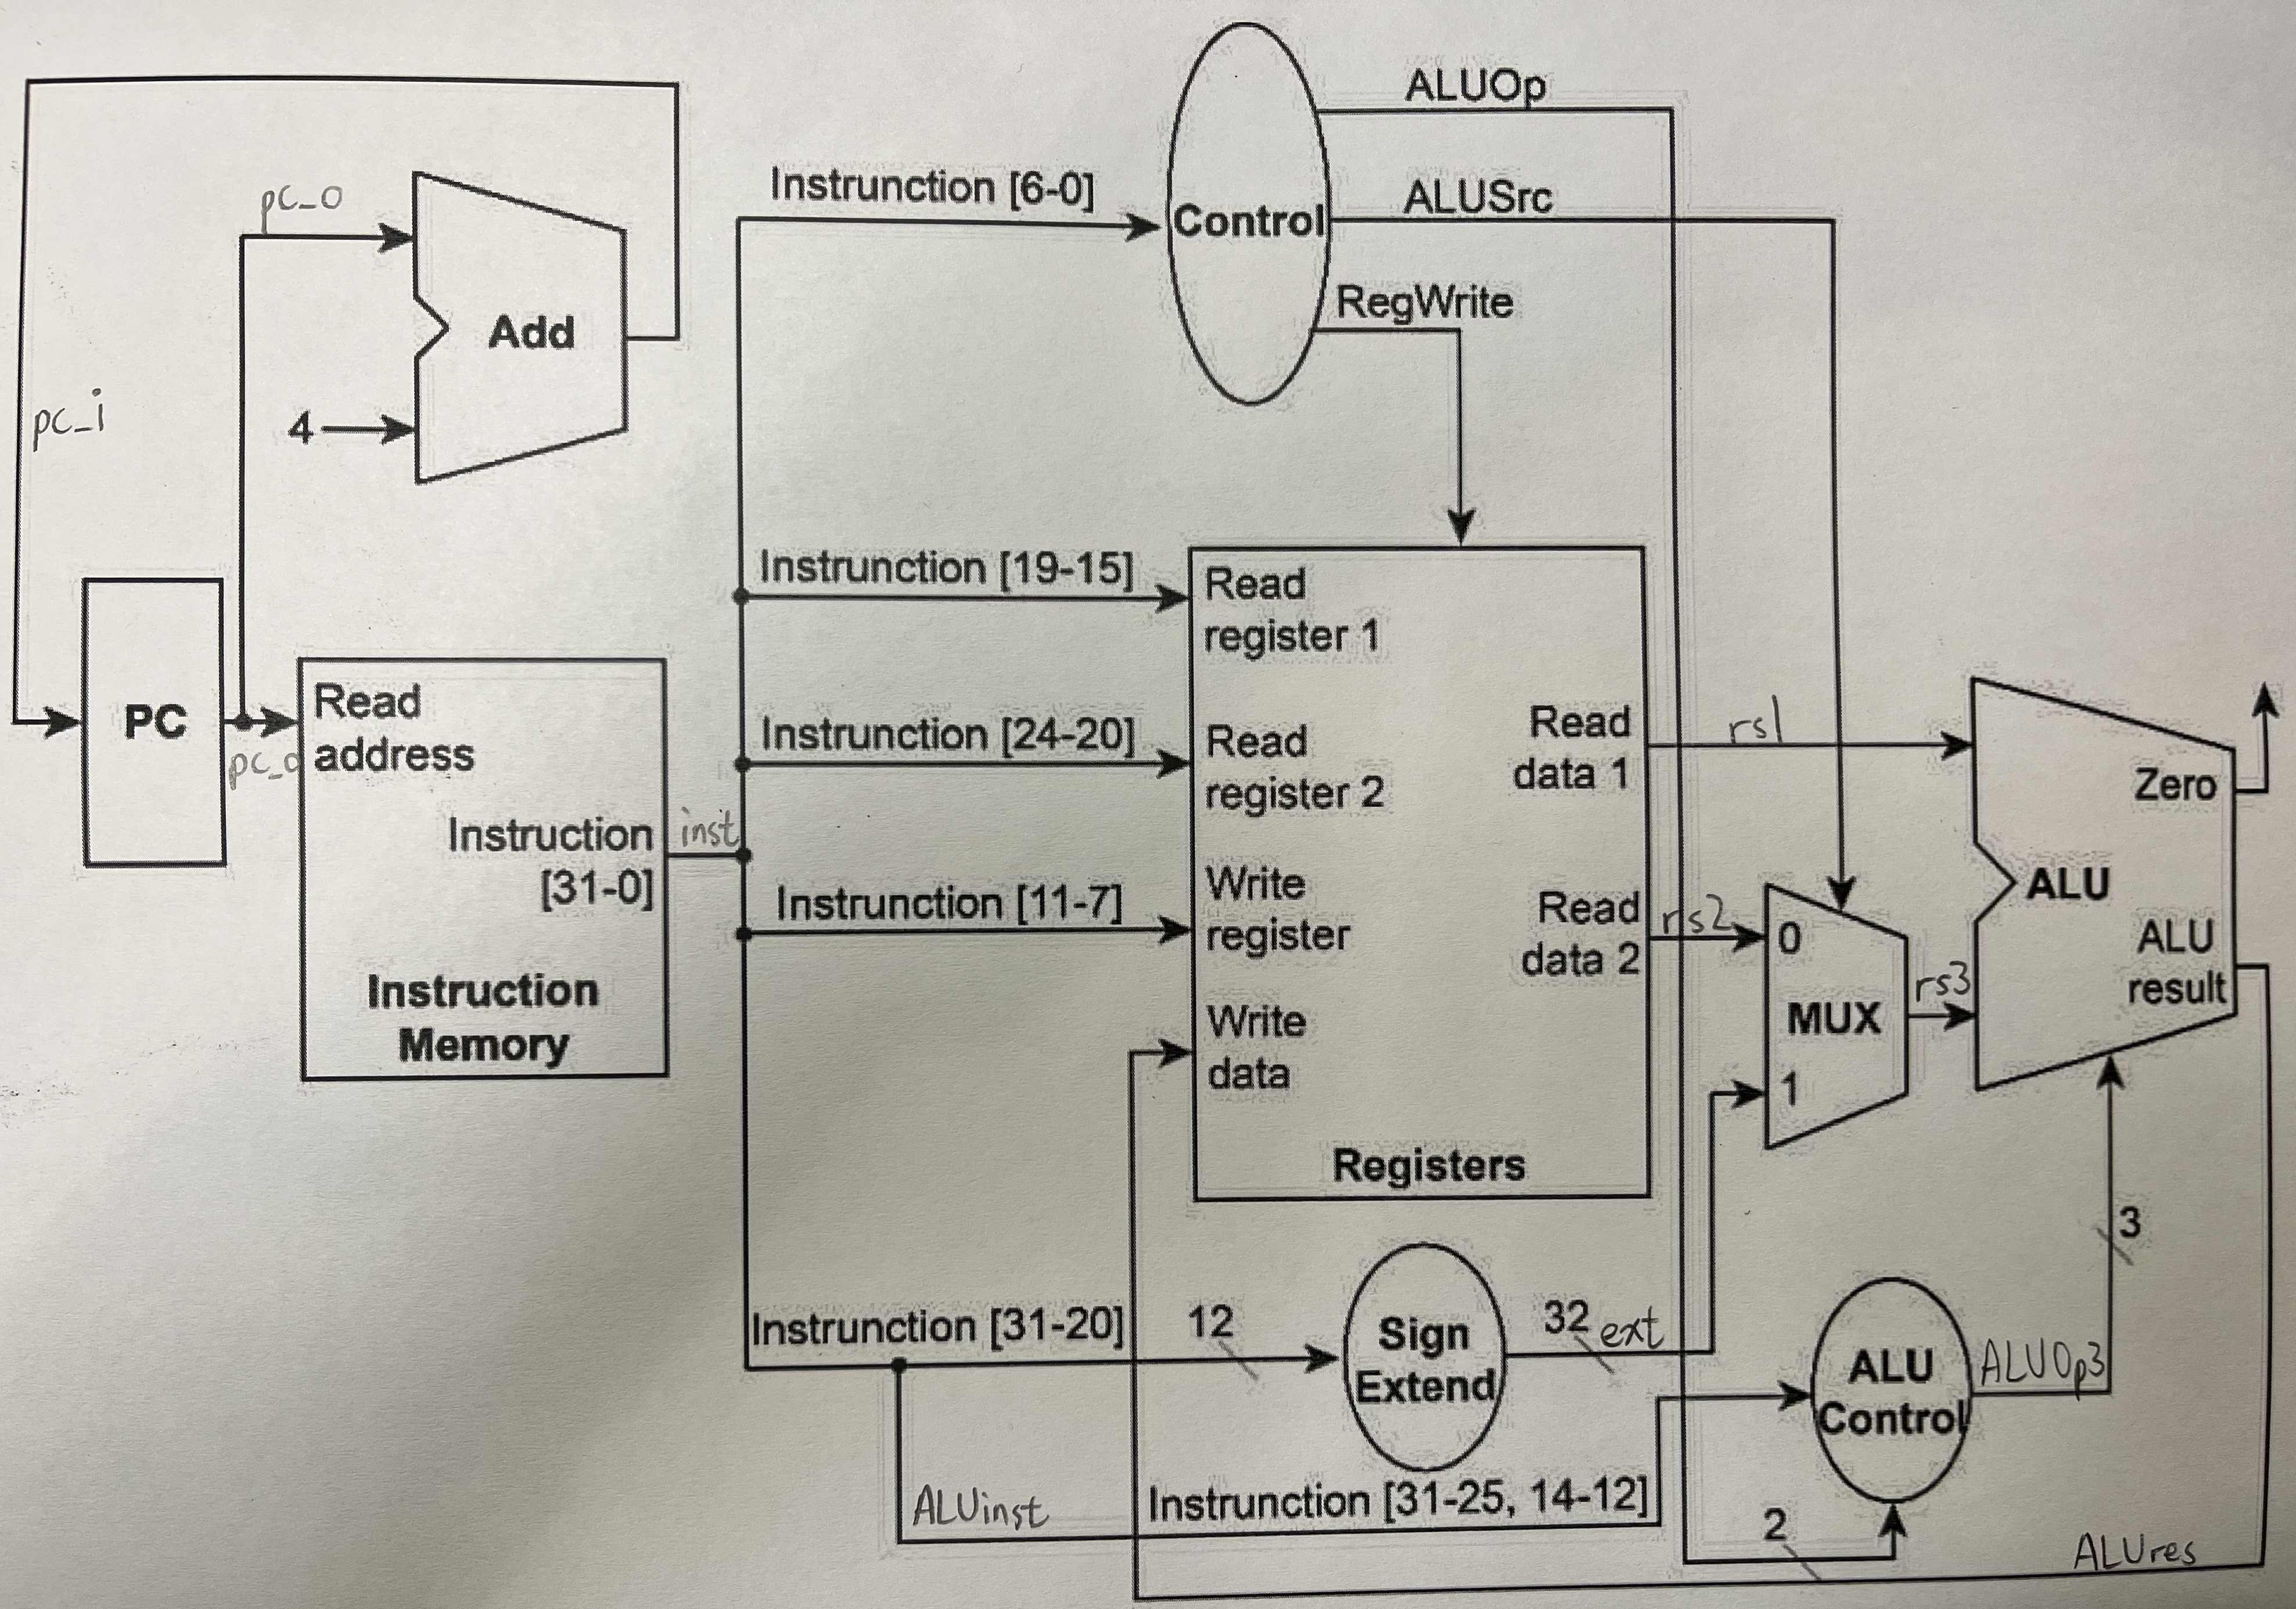
\includegraphics[width=15cm]{all.JPG}

\section{Development Environment}

\begin{itemize}
\item OS: Ubuntu 22.04.2 LTS
\item Compiler: iverilog
\end{itemize}
